\chapter{Looking Forward}

\section{Graph Matching}

\subsection{More Efficient Implementation}

While the graph matching algorithm is already an approximation, it is still not fast enough to support the pattern learning model to learn in very large scale. Therefore, a more efficient implementation is of interest from an engineering view point and if we want to move the algorithm to production system.\\

One major time sink of the algorithm is the iterative row and column normalizations enforcing by the two-way constraints. A potential solution would be using GPU to perform row/column normalization independently in parallel fashion. Another solution would be ignoring the normalizations altogether, and incorporating the two-way constraints into our objective functions with Lagrange multipliers:

\begin{align}
E(M)=&-\frac{1}{2}\sum_{a=1}^{G}\sum_{i=1}^{G'}\sum_{b=1}^{G}\sum_{j=1}^{G'}M_{ai}M_{bj}C_{abij}\nonumber\\
&-\frac{1}{\beta}\sum_{a=1}^{G}\sum_{i=1}^{G'}M_{ai}(\text{log}M_{ai}-1)\nonumber\\
&+\sum_{a=1}^{G}\mu_a(\sum_{i=1}^{G'}M_{ai}-1)+\sum_{i=1}^{G'}\nu_a(\sum_{a=1}^{G}M_{ai}-1)
\end{align}

and we can directly derive $M$ via the objective function using library like Theano\footnotemark. However, because of the nested sum, even though there is a matrix operation that can help us do the forward calculation, the back-propagation/derivation has not been implemented yet. Therefore, we did not implement such solution, but it would be much more efficient once the derivation for such operations are implemented.\\
\footnotetext{http://www.deeplearning.net/software/theano/}

Another time and memory sink for the algorithm would be the compatibility between edges. While the computation can be speed up via parallel computing, there are lots of communication overhead due to the design of the edge compatibility matrix, where each row or column is associated with a single edge in the graph and result in a $(|G|*|G|)\times(|G'|*|G'|)$ matrix. Since MATLAB only allows parallel computing row by row or column by column, we are still copying a huge vector in parallel task which result in lots of communication overhead. In addition, the compatibility matrix is very huge and could result in memory issue. Even though we can fix by storing it as a sparse matrix, sparse matrix could also introduce lots of computation overhead during the graduated assignment process.\\

Therefore, it would be beneficial for us to think of another representation for edge compatibility scores that are both memory and computation efficient.

\subsection{Automate Parameters Tuning}

A lot of the frustrations during the development of this algorithm coming from tuning the parameter considering the large number of different combinations of parameter. Considering different application of the same algorithm could have very different optimal parameters configuration, it would be beneficial for users if the algorithm has some mechanisms to tune the parameter automatically based on the expected matching result.\\

While this problem can easily turn into another project about model learning, we can start from a simple grid search, or learn about how different parameters could affect different aspects of the matching result and adjust them accordingly.


\section{Pattern Learning}

\subsection{Smarter Component Initiation}

In our model, the initial components can have a huge impact on model's pattern learning quality. For instance, if the share pattern has two components but our starting components only have one of them, the model could never capture the entire pattern. Therefore, we might want to be smarter than random when initializing our model components.\\

One potential solution would be do a pairwise graph matching before picking the components, and incorporate some heuristic rules (e.g. matching result clarity, larger matching nodes etc) to help us pick the components.\\

Another solution would be introducing a mechanism allows the model to swap in random sample ARGs as new components, and switch it our if the performance does not get better.

\subsection{Component and Node Deletion}

Since we start off with sample ARGs as our components ARGs, it is important for the components ARGs to reduce themselves in order to accurately represent the share pattern. However, in many of our experiments, the node deletion is not always perfect just based on a threshold. Therefore, we might want to introduce more heuristic rules for deletion in the future. One such rule could be examining $\beta^w$ across multiple rounds, and only delete it based on a history of pattern.\\

In addition to node deletion, it would be helpful if we could delete the entire component as well since the randomly initialized components could share similar pattern, and therefore become redundant. Introducing a mechanism for component deletion not only allow us to start from a relatively large pool of components, but also help us speed up the model training. One potential way we could do this is by comparing the result of two components matching to the same sample ARG.

\subsection{Other Applications}

Besides protein structure mining, another interesting application for the pattern learning model would be computer vision, which is dominated by Neural Network nowadays.\\

Neural Network like CNN(Convolutional Neural Network) is a very effective model for object recognition because the non-linear transformation and back-propagation are able to learn features automatically and effectively. Moreover, pooling layer has been effective in handling minor variance while different filters can handle large variance like rotation\footnotemark. However, when the scene becomes more complicated, describing the relationship between multiple object for instance, CNN becomes less effective (larger model and more training data) because CNN is more effective in learning features, but less effective in modeling relationship. For instance, if we have two objects whose relationship is a certain distance (A), to recognize the same relationship after rotation (B), a CNN might need to learn an additional filter for the $45^\circ$ angle, while an ARG representation can easily recognize the rotated scene with no trouble:\\
\footnotetext{Filters might not be representing different rotations exactly but rotation certainly requires more filters to summarize more features.} 

\begin{figure}[h]
	\centering
	\captionsetup{justification=centering}
	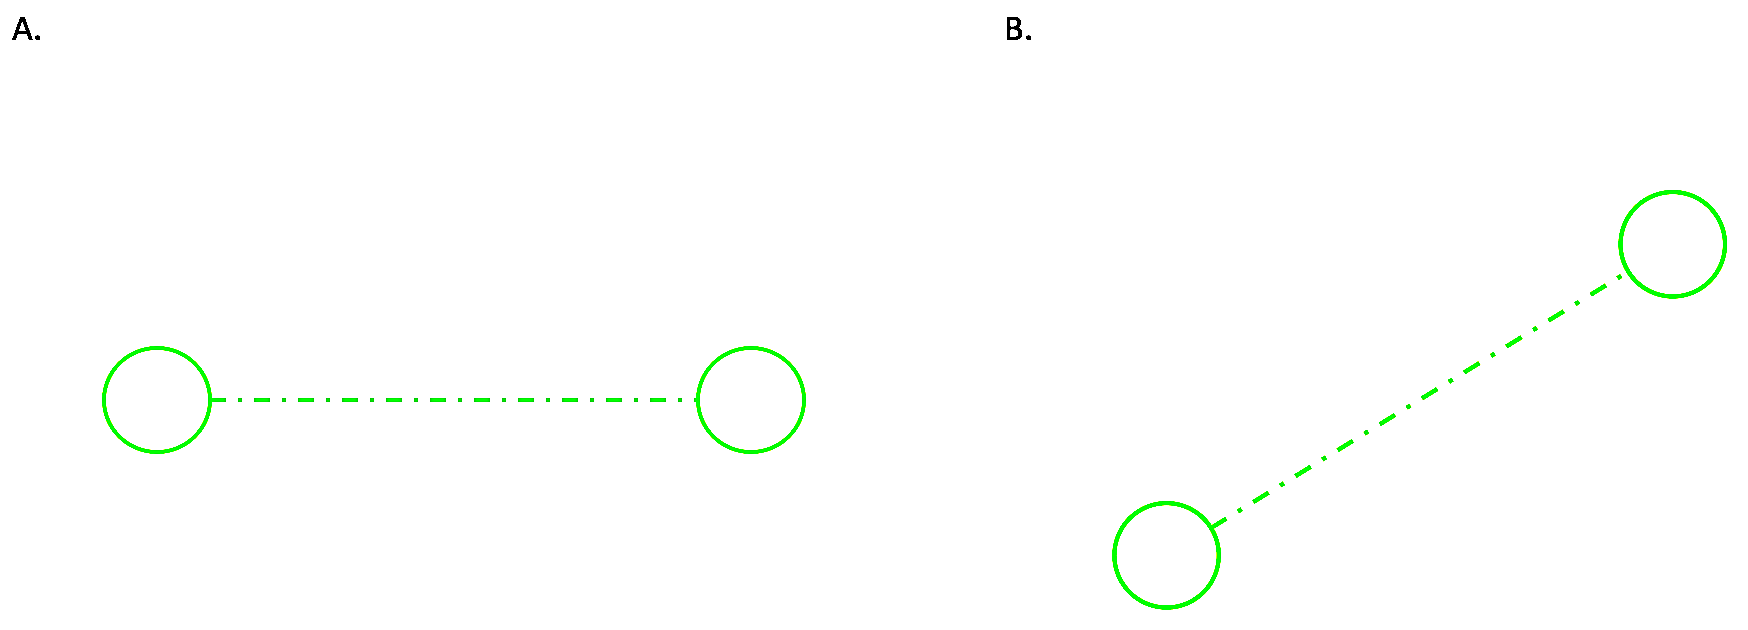
\includegraphics[width=0.8\textwidth]{figs/rotation.png}
	\caption[Caption for LOF]{\emph{A. Two objects (circles) have a relationship of a certain distance $X$.\\ B. A rotated scene showing such relationship. }}
	\label{fig:rotation}
\end{figure}

Therefore, the pattern learning model described here can be very helpful in understanding the relationship between complex scene ("student taking class", "cars stuck in traffic" etc.) while CNN helps the model to recognize individual object in the scene or generate latent representation for individual object.\\

Besides computer vision, the pattern learning model can also be used in natural language processing task, like modeling the relationship (e.g. Q\&A, extension, agreement, etc.) between sentences in a dialogues. Here, we can turn each word/concept to a node (whose label can be the word vector) and the word/concept distance as the edge. Once we turn the conversation exchange into an ARG, we might be able to model different relationship as well.\\

Therefore, combining neural network for individual object and pattern learning for modeling relationship, machines probably can learn complex structure, scenes, conversations and many other things more effectively. I am really excited about what's coming next.

\section{Protein Modeling}

\subsection{Novel Structure Motif in Protein}

While the proof of concept we did in Section \ref{sec:poc} is nice, domain discovery is not a very challenging task. Due to its relatively large size, simple 3D alignment should give you a reasonably good match and you don't really need to model the protein as an ARG.\\

However, if we are able to train the model efficiently with enough data, we might be able to discover 3D structure motifs that have long been overlooked by sequential matching algorithm. If the model can learn such novel motif, it would be of great help for many biologists.

\subsection{Protein as Documents and Amino Acid as Word}

In Section \ref{sssec:a2v}, we treated protein as documents and amino acid as word, which allows us to use model in natural language field to generate representation for amino acid.\\

In the same line, many of the models developed today in the natural language field, especially the kinds dealing with sequential model, might be a great tool for answering question about protein. For instance, we can use a Seq2Seq model to predict structure of protein sequence, or use LSTM model to predict protein chemical property with the protein sequence.


\subsection{Edge for Protein ARG Revisit}

While tuning hyper parameters for the model, we realized that the node compatibility needs to play a more important role(larger $\alpha$) in order to get clear and correct result for graph matching. This makes sense because protein alignment should be driven more by the amino acid compatibility. However, can we give edge here a different representation and a more effective relationship to help with matching/alignment?

